%%This is a very basic article template.
%%There is just one section and two subsections.
\documentclass[a4paper, 11pt]{article}
\usepackage[ngerman]{babel}
\usepackage[T1]{fontenc}
\usepackage[utf8]{inputenc} 
\usepackage{amsthm,amsfonts,amssymb,amsmath,amsbsy}
\usepackage{ngerman}
\usepackage{hyperref}
\usepackage{amsthm}
\usepackage{graphicx}
\usepackage{listings}
\usepackage{pdflscape}

\pagestyle{empty}
\author{Sarah Lutteropp, Parto Karwat}
\title{Basispraktikum Hardwarenaher Systementwurf WS 11/12 \\ Arbeitsbericht 2}
\date{\today}

\theoremstyle{definition}
\newtheorem{definition}{Definition}
\theoremstyle{plain}
\newtheorem{satz}{Satz}

\begin{document}

\maketitle

\section{Vorwort}
In diesem Aufgabenblatt ging es darum, Kenntnisse über den Umgang mit FPGAs zu erlangen und sich mit Xlinx vertraut zu machen sowie einen Überblick über verschiedene Hardwarebeschreibungssprachen zu erlangen.

\section{Xilinx ISE}
Wie haben in Xilinx unser aus dem letzten Aufgabenblatt erstelltes mynand.vhd importiert, die Pins zugeordnet und den Bitstream generiert. Anschließend haben wir erfolgreich den Bitstream auf die FPGA-Karte gespielt und unsere NAND-Schaltung mithilfe der LED und 2 Schaltern getestet. 
Siehe Source.

\section{LED-Test}
\subsection{Gesamtschaltung}
Hier ein Überblick über unsere Gesamtschaltung. Die blauen Werte stehen für die im Quelltext verwendeten Signale.
\newline
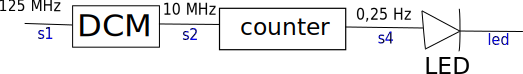
\includegraphics[width=1\textwidth]{partosBild.pdf}

\subsection{Digital Clock Manager (DCM)}
Wir haben die DCM so eingestellt, dass wir eine Ausgangsfrequenz von 10 MHz erhalten. (CLKFX ausgewählt, $M=2$, $D=25$)

\subsection{Zähler}
Wurde eingefügt. (Siehe angefügte Dateien `counter.vhd' `ledTest.vhd' und `ledTest\_tb.vhd')
Den Wert $ANZAHL$, den der Zähler hochzählt, haben wir folgendermaßen bestimmt:
$$f=\frac{1}{T}, \quad T=4 s, f_{LED} = 0.25 Hz, f_{DCM} = 10 Mhz = 10 \cdot 10^6 Hz$$
$$ f_{LED} = \frac{f_{DCM}}{2 \cdot ANZAHL}$$
$$\Rightarrow ANZAHL = 2 \cdot 10^7 = 20000000$$

\section{Synthese}
Siehe angefügte Datei `in1\_out1\_myLEDtest.ucf'. Anschließend haben wir den Bitstream generiert, auf die FPGA-Karte übertragen. Die Blinkzeit der LED betrug, wie erwartet, zwei Sekunden.

%Man unterscheidet Hardwarebeschreibungssprachen, ob sie für analoge und digitale Schaltkreise verwendet werden sollen.
%\vspace{1cm}

\begin{landscape}
\section{Hardwarebeschreibungssprachen}
\begin{tabular}{p{2cm}|p{3cm}|p{3cm}|p{3cm}|p{3cm}|p{3cm}|p{3cm}}
 & \textbf{Verilog} & \textbf{VHDL} & \textbf{SystemC} & \textbf{ParC} & \textbf{JHDL} & \textbf{Lola}\\
\hline 
Einsatz & Spezifikation und Entwurf kompletter Systeme & Spezifikation und Entwurf kompletter Systeme & noch nicht in großen wirtschaftlichen Projekten eingesetzt & Multicore und verteilte Systeme, RF/Wireless, Neuronale Netze & selbstkonfigurierende Systeme & Synchrone, digitale Schaltkreise \\
\hline
basierend auf & C & ADA & C++ & C++ & Java & PASCAL, Niklaus Wirth \\
\hline
Vorteile & leichter erlernbar als VHDL, schnelle, simple Umsetzung, Einflussmöglichkeiten auf der Gatterebene (UDP), keine strenge Typprüfung & großer Sprachschatz, höher angesiedelt (bis zur Systemebene), starke Typisierung, Wiederverwendbarkeit, Vielseitigkeit,  & schnelle Simulationen, nahtloser Top-Down-Entwurf & kann als Basis für KI verwendet werden (Neuronale Netze), kann dynamisch erzeugt werden & kostenlos, leicht konfigurierbar, leicht erweiterbar & einfach, leicht erlernbar \\
\hline
Nachteile & geringerer Sprachschatz als VHDL & schwerer erlernbar als Verilog, enthält Konstrukte, die sich nicht auf Hardwareebene realisieren lassen & syntaktischer Overhead, mangelnde Angebot an Synthesewerkzeugen, kein Powermanagement & geringe Verbreitung & JVM benötigt, auf Linux braucht man Wine zur Bitstreamgenerierung & keine Anwendung in der Industrie, geringer Sprachschatz \\
\end{tabular}


\begin{tabular}{p{2cm}|p{3cm}|p{3cm}|p{3cm}|p{3cm}|p{3cm}|p{3cm}}
 & \textbf{Verilog} & \textbf{VHDL} & \textbf{SystemC} & \textbf{ParC} & \textbf{JHDL} & \textbf{Lola}\\
\hline 
Verbreitungs- grad & sehr hoch, weltweit, insbesondere USA & sehr hoch, bedeutendste HDL in Europa & De-facto-Standard im Bereich IP-Nutzung und System-Level-
Spezifikation & gering & gering & nur in der Lehre (ETH Zürich), sehr gering\\
\hline
Synthese- programme & Xilinx, Icarus Verilog, Quartus II \ldots & Xilinx, Synplify Pro, \ldots & SystemC-Compiler von Synopsys
 & - & Xilinx & -\\
\hline
Sonstiges & ursprünglich Simulationssprache, seit 1995 IEEE-Standard, lange Zeit herstellerspezifisch & seit 1987 IEEE-Standard, von Beginn an als offener Standard entwickelt & Firmenunter- stützung bei Weiterentwicklung, Spracherweiterung & Teil des V2000 open simulator project, 1:1 - Mapping, Spracherweiterung & Open-Source, Spracherweiterung & - \\
\hline
Entwurfsjahr & 1983/84 & 1985 (erste kommerzielle Version) & 1999 & - & 1997 & 1994
\end{tabular}
\end{landscape}


\end{document}